\documentclass[paper=a4, fontsize=11pt]{scrartcl}
\usepackage{mathtools}
\DeclarePairedDelimiter\ceil{\lceil}{\rceil}
\DeclarePairedDelimiter\floor{\lfloor}{\rfloor}
\usepackage[T1]{fontenc}
\usepackage[english]{babel}
\usepackage{listings}
\usepackage{amsmath,amsfonts,amsthm,mathrsfs}
\usepackage{sectsty} % Allows customizing section commands
\allsectionsfont{\centering \normalfont\scshape} % Make all sections centered, the default font and small caps
\usepackage{fancyhdr} % Custom headers and footers
\pagestyle{fancyplain} % Makes all pages in the document conform to the custom headers and footers
\fancyhead{} % No page header - if you want one, create it in the same way as the footers below
\lstset{
  breaklines=true
}
\fancyfoot[L]{} % Empty left footer
\fancyfoot[C]{} % Empty center footer
\fancyfoot[R]{\thepage} % Page numbering for right footer
\renewcommand{\headrulewidth}{0pt} % Remove header underlines
\renewcommand{\footrulewidth}{0pt} % Remove footer underlines
\setlength{\headheight}{13.6pt} % Customize the height of the header
\numberwithin{equation}{section} % Number equations within sections (i.e. 1.1, 1.2, 2.1, 2.2 instead of 1, 2, 3, 4)
\numberwithin{figure}{section} % Number figures within sections (i.e. 1.1, 1.2, 2.1, 2.2 instead of 1, 2, 3, 4)
\numberwithin{table}{section} % Number tables within sections (i.e. 1.1, 1.2, 2.1, 2.2 instead of 1, 2, 3, 4)
\setlength\parindent{0pt} % Removes all indentation from paragraphs - comment this line for an assignment with lots of text
\newtheorem*{solution}{Solution}

\newcommand{\horrule}[1]{\rule{\linewidth}{#1}} % Create horizontal rule command with 1 argument of height

\title{	
\normalfont \normalsize 
\textsc{Dept. of Computer Science, University of California, Davis\\ECS152 \hspace{.5in}
%%%%%%%%%%%%%%%%%%%%%%%%%%%%
%%%% Add your name here %%%%
%%%%%%%%%%%%%%%%%%%%%%%%%%%%
Weiran Guo(912916431) \hspace{.5in} \today}
\horrule{0.5pt} \\[0.4cm]
%%%%%%%%%%%%%%%%%%%%%%%%%%%%%%%%%%%%
%%%% Write the Homework # here %%%%%
%%%%%%%%%%%%%%%%%%%%%%%%%%%%%%%%%%%%
\huge Project2 Report \\
\horrule{2pt} \\[0.5cm]
}

\date{}

\begin{document}

\maketitle

\vspace{-1in}


\section{Part 1}

       a).\\
       if the number of packets in the system less than B, %$\floor*{\frac{B}{\lambda}}$,
       then the packet loss won't happens.\\
       
        %\begin{equation}
            %N = \floor*{\frac{B}{\lambda}}\\
        %\end{equation}
        for markov chain, the maximum packet in the system is B, hence,
        \begin{align}
            \lambda\pi_0 &= \mu\pi_1\\
            \lambda\pi_1 &= \mu\pi_2\\
                &...\\
            \lambda\pi_{B} &= \mu\pi_{B+1}\\
        \end{align}
        therefore,
        \begin{align}
            1 &= \sum_{i = 0}^{B+1} \pi_i\\
            1 &= \sum_{i = 0}^{B+1} \pi_0(\frac{\lambda}{\mu}^i)\\
            \pi_0 &= \frac{1-\frac{\lambda}{\mu}}{1-\frac{\lambda}{\mu}^{B+1}}\\
            \pi_{B+1} &= \frac{\frac{\lambda}{\mu}^{B+1}(1-\frac{\lambda}{\mu})}{1-\frac{\lambda}{\mu}^{B+2}}\\
        \end{align}
        hence, the loss rate is
        \begin{equation}
            P_d = \frac{\frac{\lambda}{\mu}^{B+1}(1-\frac{\lambda}{\mu})}{1-\frac{\lambda}{\mu}^{B+2}}\\
        \end{equation}

       b).simulation code\\
       \begin{lstlisting}[language=Python]
# This is a simpy based  simulation of a M/M/1 queue system
# Now the buffer packet size is limited to B

import random
import simpy
import math

RANDOM_SEED = 29
SIM_TIME = 1000000
MU = 1



""" Queue system  """		
class server_queue:
	def __init__(self, env, arrival_rate, Packet_Delay,
	Server_Idle_Periods, Buffer_Size):
		self.server = simpy.Resource(env, capacity = 1)
		self.env = env
		self.queue_len = 0
		self.flag_processing = 0
		self.packet_number = 0
		self.sum_time_length = 0
		self.start_idle_time = 0
		self.drop = 0
		self.buffer_size = Buffer_Size
		self.arrival_rate = arrival_rate
		self.Packet_Delay = Packet_Delay
		self.Server_Idle_Periods = Server_Idle_Periods
		
	def drop_rate(self):#calculate the drop rate, drop/total_packets
		return self.drop/self.packet_number
    
	def process_packet(self, env, packet):
		with self.server.request() as req:
			start = env.now
			yield req
			yield env.timeout(random.expovariate(MU))
			latency = env.now - packet.arrival_time
			self.Packet_Delay.addNumber(latency)
			#print("Packet number {0} with arrival time {1} latency {2}".format(packet.identifier, packet.arrival_time, latency))
			self.queue_len -= 1
			if self.queue_len == 0:
				self.flag_processing = 0
				self.start_idle_time = env.now
				
	def packets_arrival(self, env):
		# packet arrivals 
		
		while True:
		     # Infinite loop for generating packets
			yield env.timeout(random.expovariate(self.arrival_rate))
			  # arrival time of one packet
			self.packet_number += 1
			  # packet id
			arrival_time = env.now  
			#print(self.num_pkt_total, "packet arrival")
			new_packet = Packet(self.packet_number,arrival_time)
			if self.flag_processing == 0:
				self.flag_processing = 1
				idle_period = env.now - self.start_idle_time
				self.Server_Idle_Periods.addNumber(idle_period)
				#print("Idle period of length {0} ended".format(idle_period))
			if self.queue_len < self.buffer_size:#######drop packet
				self.queue_len += 1
				env.process(self.process_packet(env, new_packet))
			else:
				self.drop += 1


""" Packet class """			
class Packet:
	def __init__(self, identifier, arrival_time):
		self.identifier = identifier
		self.arrival_time = arrival_time
		

class StatObject:
    def __init__(self):
        self.dataset =[]

    def addNumber(self,x):
        self.dataset.append(x)
    def sum(self):
        n = len(self.dataset)
        sum = 0
        for i in self.dataset:
            sum = sum + i
        return sum
    def mean(self):
        n = len(self.dataset)
        sum = 0
        for i in self.dataset:
            sum = sum + i
        return sum/n
    def maximum(self):
        return max(self.dataset)
    def minimum(self):
        return min(self.dataset)
    def count(self):
        return len(self.dataset)
    def median(self):
        self.dataset.sort()
        n = len(self.dataset)
        if n//2 != 0: # get the middle number
            return self.dataset[n//2]
        else: # find the average of the middle two numbers
            return ((self.dataset[n//2] + self.dataset[n//2 + 1])/2)
    def standarddeviation(self):
        temp = self.mean()
        sum = 0
        for i in self.dataset:
            sum = sum + (i - temp)**2
        sum = sum/(len(self.dataset) - 1)
        return math.sqrt(sum)

def cal_packet_loss(arrival_rate, buffer_size):#######the theoretical loss rate
    pd = 1 - (1 - (arrival_rate/MU)**buffer_size)/(1 - (arrival_rate/MU)**(buffer_size+1))
    #print(Sum)###########each step print out the calculated probability that the packet of system is <= buffer size
    
    return pd

def main():
    random.seed(RANDOM_SEED)
    for buffer_size in [10, 50]:
        print("Simple queue system model:mu = {0}, buffer size = {1}".format(MU, buffer_size))
        print ("{0:<9} {1:<9} {2:<9} {3:<9} {4:<9} {5:<9} {6:<9} {7:<9} {8:<9} {9:<9}".format(
        "Lambda", "Count", "Min", "Max", "Mean", "Median", "Sd", "Utilization", "Loss Rate", "Theoretical"))
        for arrival_rate in [0.2, 0.4, 0.6, 0.8, 0.9, 0.99]:
            env = simpy.Environment()
            Packet_Delay = StatObject()
            Server_Idle_Periods = StatObject()
            router = server_queue(env, arrival_rate, Packet_Delay, Server_Idle_Periods, buffer_size)
            env.process(router.packets_arrival(env))
            env.run(until=SIM_TIME)
            #expected_delay = 1/MU/(1-(arrival_rate/MU))
            print ("{0:<9.3f} {1:<9} {2:<9.3f} {3:<9.3f} {4:<9.3f} {5:<9.3f} {6:<9.3f} {7:<9.3f} {8:<9.3f} {9:<9.3f}".format(
                round(arrival_rate, 3),
                int(Packet_Delay.count()),
                round(Packet_Delay.minimum(), 3),
                round(Packet_Delay.maximum(), 3),
                round(Packet_Delay.mean(), 3),
                round(Packet_Delay.median(), 3),
                round(Packet_Delay.standarddeviation(), 3),
                round(1-Server_Idle_Periods.sum()/SIM_TIME, 3),
                round(router.drop_rate(),3),
                round(cal_packet_loss(arrival_rate, buffer_size),3)))

if __name__ == '__main__': main()
       \end{lstlisting}
       c).tables\\
        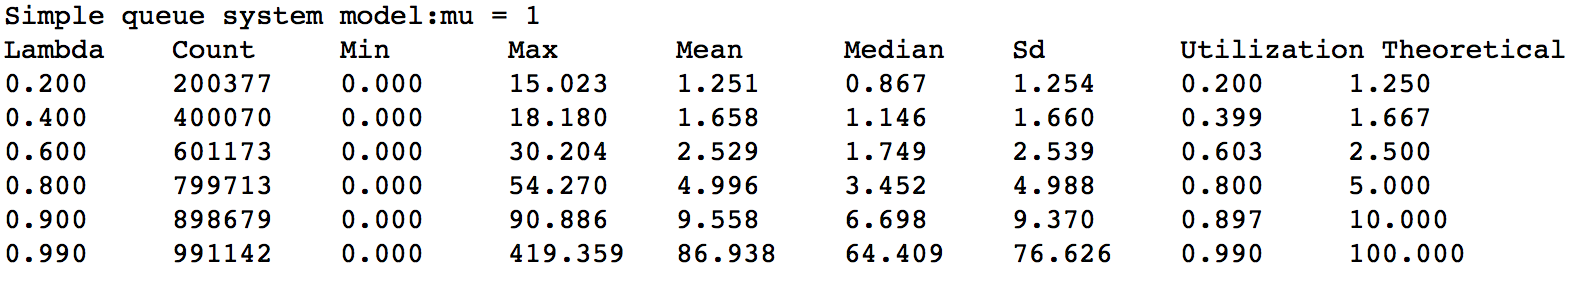
\includegraphics[scale=0.5]{b}\\\\
        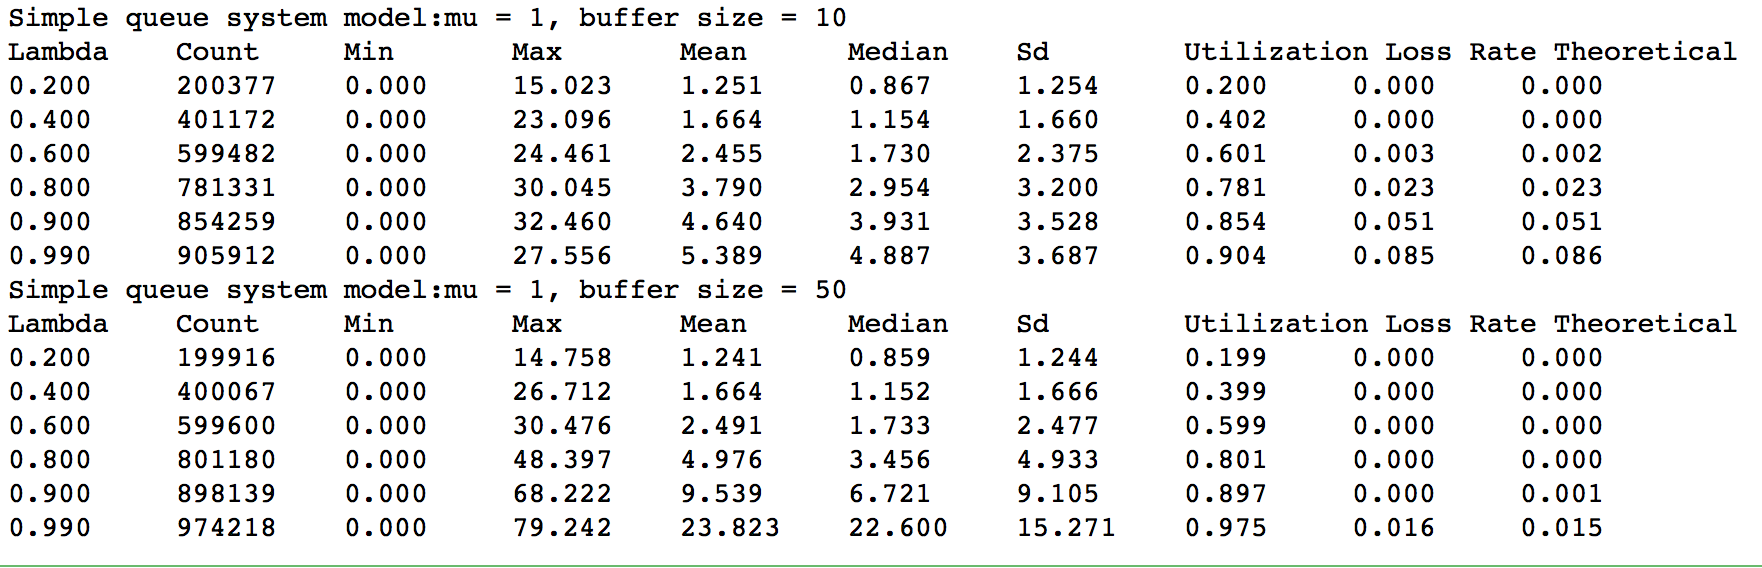
\includegraphics[scale=0.5]{a}
    
\section{Part 2}
    a). Sample execution\\
    \begin{lstlisting}[language=Python]
    """Binary Exponetial and Linear Backoff Algorithm"""

import random
import simpy
import math

RANDOM_SEED = 29
SIM_TIME = 1000000
MU = 1
TS = 1 #time slot
N_HOST = 3 #number of hosts

""" Host class """
class Host:
    def __init__(self, env, arrival_rate):
        self.env = env
        self.arrival_rate = arrival_rate
        self.L = 0
        self.S = 0
        #self.arrives = 0
        self.N = 0 #times retransmitted
        self.server = simpy.Resource(env, capacity = 1)
        env.process(self.packets_arrival(env))
        
    def packets_arrival(self, env):
        while True:
            yield env.timeout(random.expovariate(self.arrival_rate))
            #self.arrives += 1
            if (self.L == 0): #no packet in the queue
                self.S = math.floor(env.now) + 1
                self.N = 0
            self.L += 1
        
    def process_packet(self, env):
        self.L -= 1
        if (self.L > 0):
            self.N = 0
            self.S = math.floor(env.now) + 1
    
    def exp_backoff(self, env):
        r = min(self.N, N_HOST)
        self.S = math.floor(env.now + random.randint(0,2**r)*TS) + 1
        self.N += 1
        
    def linear_backoff(self, env):
        K = min(self.N, 1024)
        self.S = math.floor(env.now + random.randint(0, K)*TS) + 1
        self.N += 1

""" Queue system  """		
class Ethernet:
    def __init__(self, env, arrival_rate, Type):
        self.env = env
        self.hosts = [Host(env, arrival_rate) for i in range(N_HOST)]
        self.success = 0
        self.collide = 0
        self.blank = 0
        self.Type = Type 
        self.arrival_rate = arrival_rate

    def sim(self, env):
        while True:
            hostLst = []
            for host in self.hosts:
                if (host.L > 0 and (host.S == math.floor(env.now))):#host is requesting now
                    hostLst.append(host)
            #print(len(hostLst))
            if (len(hostLst) == 1):#succeed
                hostLst[0].process_packet(env)
                self.success += 1
            elif (len(hostLst) > 1):#collide
                self.collide += 1
                for host in hostLst:
                    if (self.Type == 0):#exponetial
                        host.exp_backoff(env)
                    else:
                        host.linear_backoff(env)
            else:
                self.blank += 1
            yield self.env.timeout(TS)
                

def main():
	print("Ethernet system model:mu = {0}, Ts = {1}, N = {2}".format(MU, TS, N_HOST))

	random.seed(RANDOM_SEED)
	for Type in [0,1]:
		if (Type == 0):
			print ("For Exponetial Backoff Algorithm")
		else:
			print ("For Linear Backoff Algorithm")
		print ("{0:<9} {1:<9} {2:<9} {3:<9} {4:<9}".format(
			"Lambda", "Success", "Failed","Blank", "Throughput"))
		for arrival_rate in [0.01, 0.02, 0.03, 0.04, 0.05, 0.06, 0.07, 0.08, 0.09]:
			env = simpy.Environment()
			ethernet = Ethernet(env, arrival_rate, Type)
			env.process(ethernet.sim(env))
			env.run(until=SIM_TIME)
			print ("{0:<9.3f} {1:<9} {2:<9}{3:<9} {4:<9.5f}".format(
				arrival_rate,
				ethernet.success,
				ethernet.collide,
				ethernet.blank,
				ethernet.success/SIM_TIME))
	
if __name__ == '__main__': main()
    \end{lstlisting}
    \\b).Simulation results of the 10-host system\\
        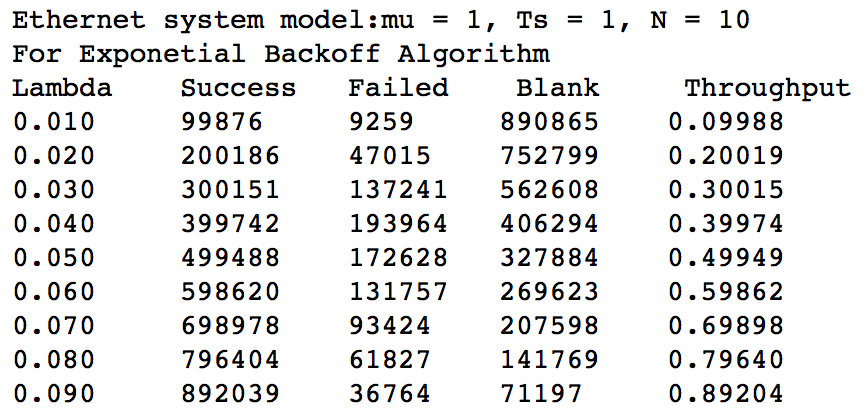
\includegraphics[scale=0.8]{c}\\\\
        for exponential backoff algorithm, as $\lambda$ increases, the Throughput increases linearly.
        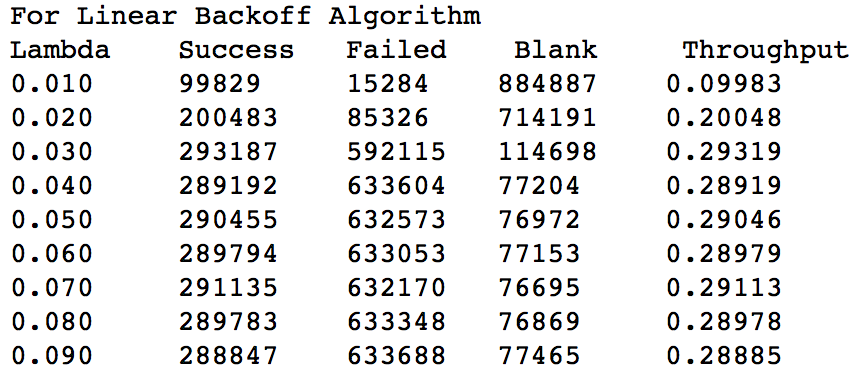
\includegraphics[scale=0.8]{d}\\\\
        for linear backoff algorithm, as $\lambda$ increases, the Throughput increases at first, but reaches the ceiling throughput around 0.29.\\\\
        Analysis: as $\lambda$ increases, for exponential backoff algorithm, the success slots keep increases until the throughput approaches 1, the blank time slots keep decreasing which means the algorithm is effective.\\
        However, the throughput of linear backoff algorithm reaches its ceiling aroung 0.29, which is not effective, that means the blank time slots does not decrease after $\lambda$ reaches certain level, while the throughput is 0.29 that far less than 1.
\end{document}